\documentclass[Bachelorarbeit.tex]{subfiles}
\begin{appendix}
\chapter{Appendix}
If not otherwise noted pictures are taken from \textit{Wikicommons}. http://commons.wikimedia.org
\addtocontents{toc}{\protect\setcounter{tocdepth}{1}}
%\ifthenelse{\equal{\getLanguage}{english}} % %prints just the list of acronyms
%  		{\addcontentsline{toc}{chapter}{Appendix}}
%  		{\addcontentsline{toc}{chapter}{Anhang}} 
\section{YCbCr-Color-Space}  	
\subsection{Procedure}
\subsection{Examples}

\newpage

\section{Color threshold}  	
\subsection{Procedure}
According to different literature (Real Time Detection and Tracking of Human Face using Skin Color Segmentation and Region Properties \cite{RTFaceDetection}, Face Detection Using Color Thresholding, and Eigenimage Template Matching \cite{RTFaceDetection} and A Robust Skin Color Based Face Detection Algorithm \cite{RobustSkinColorFD}) the thresholds must be found with an try and error procedure.

The three mentioned articles have chosen different thresholds, in this project the thresholds were chosen with the MATLAB application colorThresholder (from the Image Processing Toolbox).

\medskip
To run this application the command \textit{colorThresholder} must be entered into the command window of MATLAB.

\medskip
After loading an image and choosing the color space (in this case the YCbCr space - see figure \ref{obamaOrig}) the thresholds can be set (see figure \ref{obamaThres}).

The next step is to use the find values for Cb and Cr:
\begin{itemize}
\item Cb: 105 $>$ Cb $<$ 120
\item Cr: 140 $>$ Cr $<$ 165
\end{itemize}

to threshold the image (values above the over limit and pixel values under the lower value will be set to black, all pixels within the limit will set to white). This can be done with the matlab commands:
\begin{lstlisting}
% Thresholding -> binary
thresh_cb = cb > 105 & cb < 120;    % thresholding for cb values
thresh_cr = cr > 140 & cr < 165;    % thresholding for cr values
binary_pic = thresh_cb&thresh_cr;   % create binary picture
\end{lstlisting}
The result looks like figure \ref{obamaBin}.

\medskip
The next steps is to modify the binary picture (by removing the small black pixels in the face and the small white pixels out of the face) to make face detection more efficient.

\begin{figure}[!h]
\centering
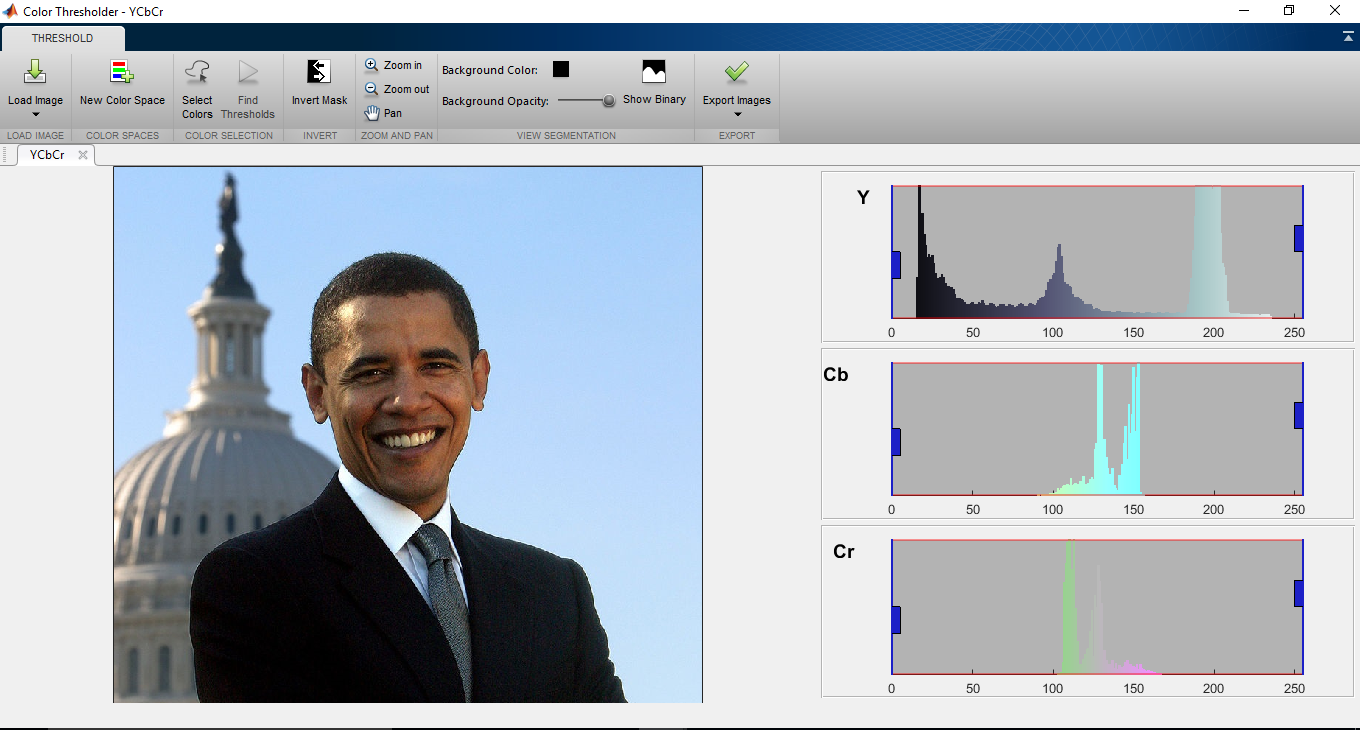
\includegraphics[width=5cm]{./img/thresholds/obama_orig.PNG}
\caption{colorThresholder - Barrack Obama - without thresholding}
\label{obamaOrig}
\end{figure}

\begin{figure}[!h]
\centering
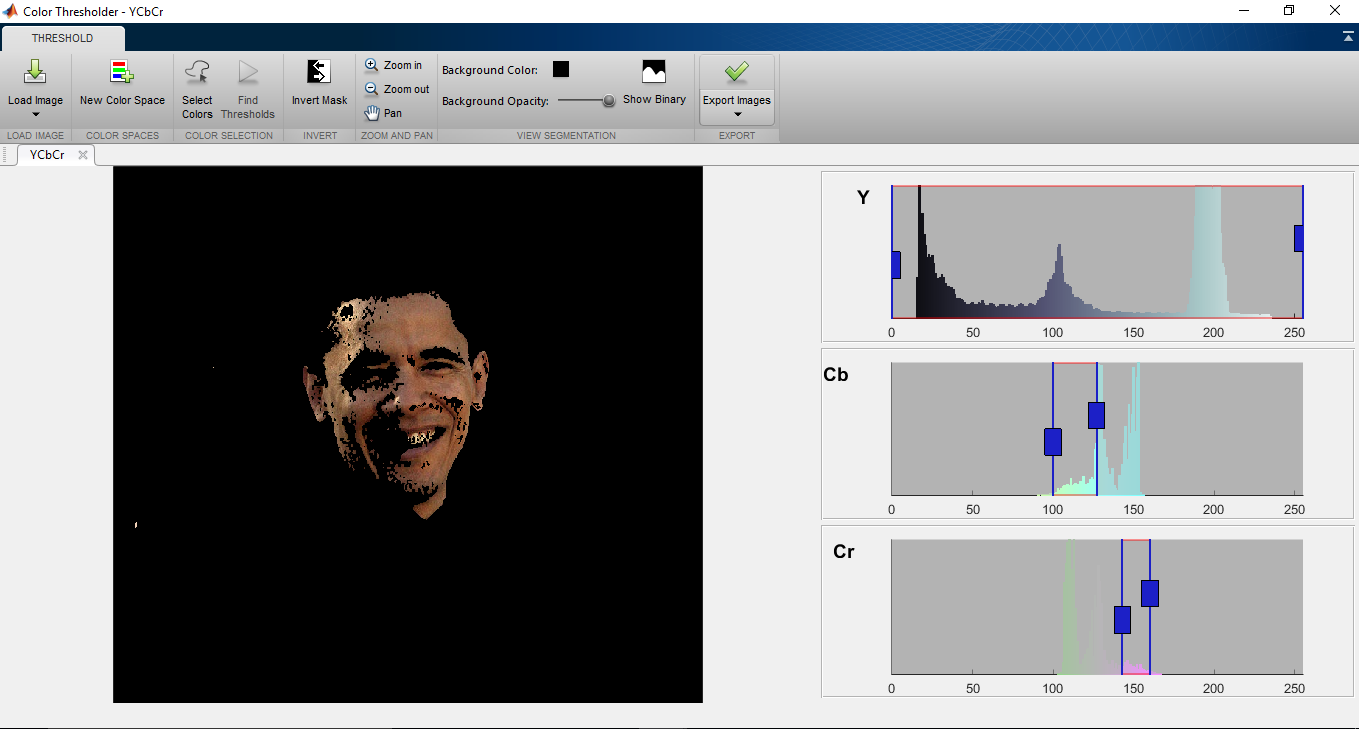
\includegraphics[width=10cm]{./img/thresholds/obama_thresholds.PNG}
\caption{colorThresholder - Barrack Obama - with thresholds : 105 $>$ cb $<$ 120 and 140 $>$ cr $<$ 165}
\label{obamaThres}
\end{figure}

\begin{figure}[!h]
\centering
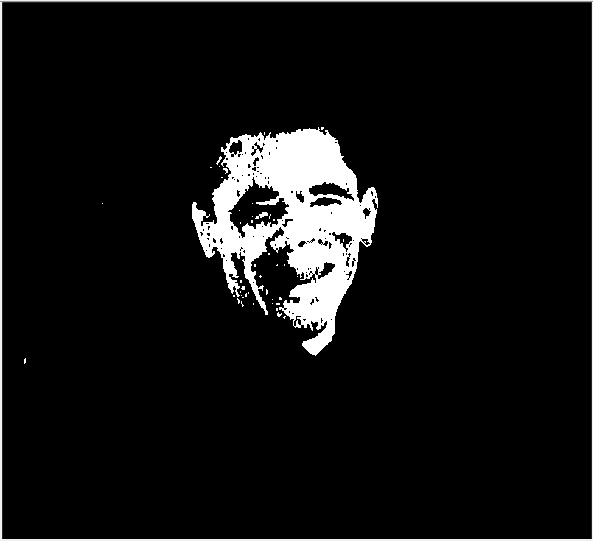
\includegraphics[width=8cm]{./img/thresholds/obama_thresholds_binary.PNG}
\caption{colorThresholder - Barrack Obama - with thresholds - Binary}
\label{obamaBin}
\end{figure}

\newpage
\subsection{MATLAB implementation}
\begin{lstlisting}[caption=Color thresholding, label= matlabColorTresholding]
I=imread('../pictures/obama.jpg');  % load image from workspace

% RGB -> YCbCr
YCBCR = rgb2ycbcr(I);               % transform image into YCbCr space
y = YCBCR(:,:,1);                   % extract Y value out of matrix
cb = YCBCR(:,:,2);                  % extract Cb value out of matrix
cr = YCBCR(:,:,3);                  % extract Cr value out of matrix

% Thresholding -> binary
thresh_cb = cb > 105 & cb < 120;    % thresholding for cb values
thresh_cr = cr > 140 & cr < 165;    % thresholding for cr values
binary_pic = thresh_cb&thresh_cr;   % create binary picture

% show binary picture:
figure
imshow(binary_pic);
\end{lstlisting}

\begin{figure}[!h]
\centering
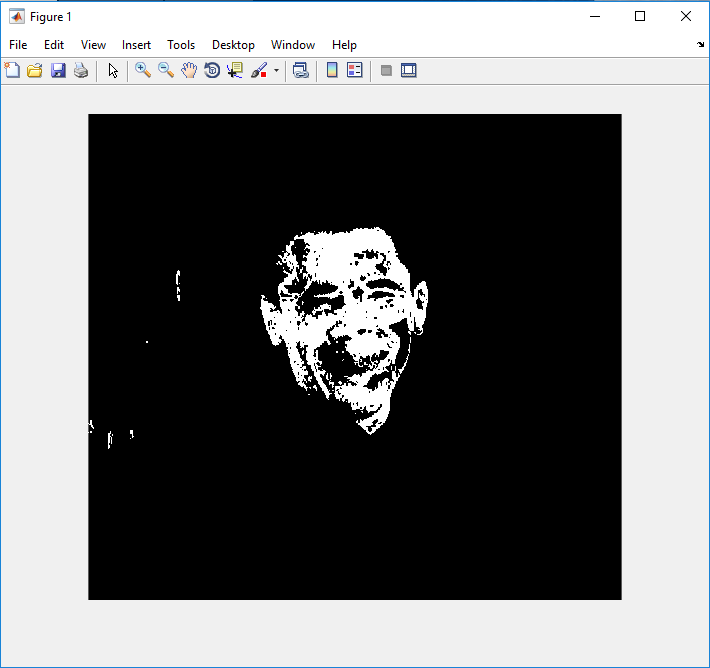
\includegraphics[width=10cm]{./img/thresholds/obama_matlab.PNG}
\caption{colorThresholder - Barrack Obama - figure out of matlab code \ref{matlabColorTresholding}}
\label{obamaThres}
\end{figure}

\subsection{Examples}

\begin{figure}[!h]
\centering
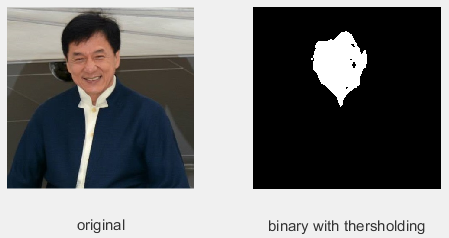
\includegraphics[height = 4cm]{./img/thresholds/chackie}
\caption{Chackie Jan}
\end{figure}

\begin{figure}[!h]
\centering
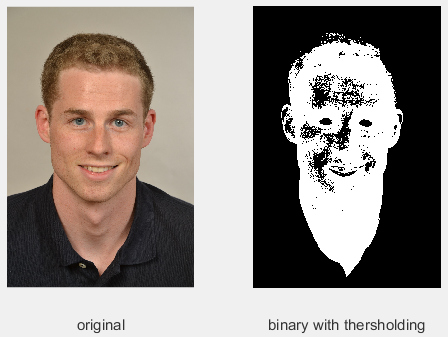
\includegraphics[height = 4cm]{./img/thresholds/tobiBu}
\caption{MEM student (private picture)}
\end{figure}
\begin{figure}[!h]
\centering
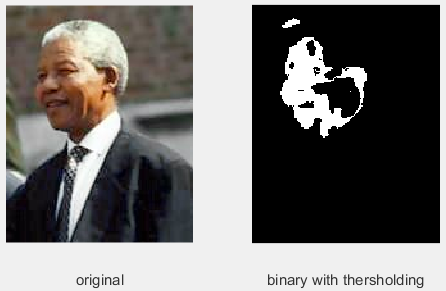
\includegraphics[height = 4cm]{./img/thresholds/mandela}
\caption{Nelson Mandela}
\end{figure}



	
\end{appendix}
